\documentclass[11pt]{article}
\def\nterm {Spring }
\def\nyear {2023}
\def\nlecturer {D. Crowdy}
\def\ncourse {Introduction to Applied Mathematics}
\def\nshort {Applied Mathematics}
\usepackage{amsmath, amsthm, amssymb, amsfonts}
\usepackage{fancyhdr}
\usepackage{xparse, xpatch}
\usepackage[svgnames]{xcolor}
\usepackage[shortlabels]{enumitem}
\usepackage[thinc,text]{esdiff}
\usepackage[bottom]{footmisc}
\usepackage[most]{tcolorbox}
\usepackage{physics}
\usepackage{tikz}
\usepackage{pgfplots}
\usepackage{graphicx, tabularx, caption}
\usepackage{csquotes}
\usepackage[a4paper, left=1.2in, right=1.2in, bottom=1in]{geometry}
\usepackage[hidelinks]{hyperref}
\hypersetup{
    colorlinks,
    allcolors=black
}
\pgfplotsset{compat=1.18}
\graphicspath{{./images/}}

% meta
\setlength{\headheight}{13.6pt}
\renewcommand*\contentsname{Outline}
\pagestyle{fancy}
\lhead{\nouppercase{\leftmark{}}}
\rhead{\nshort}
\title{\textbf{\ncourse}}
\author{Lectured by \nlecturer \\\small Notes taken by Dongshen Wu\footnote{These notes are usually modified significantly after lectures, and are not endorsed by the lecturers at Imperial College, London. They are by no means an accurate representations of what was actually lectured. In particular, all errors are almost surely mine.}}
\date{\nterm \nyear}

% centre tikz pictures
\makeatletter
\g@addto@macro\@floatboxreset\centering
\makeatother

% environment
\tcbset{
  defstyle/.style={
    enhanced, sharp corners,
    attach boxed title to top left={yshift=-2.75mm, 
      xshift=5mm, yshifttext=-2.2mm},
    colback=white, colframe=PeachPuff,
    coltitle=black, fonttitle=\bfseries,
    before skip=7pt,
    boxed title style={sharp corners, size=small,
      colback=PeachPuff,colframe=PeachPuff,}},
  thmstyle/.style={
    enhanced, sharp corners,
    attach boxed title to top left={yshift=-2.75mm, 
      xshift=5mm, yshifttext=-2.2mm},
    colback=AliceBlue, colframe=LightBlue,
    coltitle=black, fonttitle=\bfseries,
    before skip=7pt,
    boxed title style={sharp corners, size=small,
      colback=LightBlue,colframe=LightBlue,}},
  propstyle/.style={
    enhanced, sharp corners,
    attach boxed title to top left={yshift=-2.75mm, 
      xshift=5mm, yshifttext=-2.2mm},
    colback=white, colframe=PowderBlue,
    coltitle=black, fonttitle=\bfseries,
    before skip=7pt,
    boxed title style={sharp corners, size=small,
      colback=PowderBlue,colframe=PowderBlue,}},
}

\newtcbtheorem[number within=section]{TcbThm}{Theorem}{
  thmstyle}{thm}
\NewDocumentEnvironment{theorem}{ O{} O{} }
  {\TcbThm{#1}{#2}}{\endTcbThm}

\newtcbtheorem[number within=section, use counter from=TcbThm]{TcbProp}{Proposition}{
  propstyle}{prop}
\NewDocumentEnvironment{proposition}{ O{} O{} }
  {\TcbProp{#1}{#2}}{\endTcbProp}

\newtcbtheorem[number within=section,use counter from=TcbThm]{TcbDef}{Definition}{
  defstyle}{def}
\NewDocumentEnvironment{definition}{ O{} O{} }
  {\TcbDef{#1}{#2}}{\endTcbDef}

\newtcbtheorem[number within=section,use counter from=TcbThm]{TcbAxi}{Axiom}{
  defstyle}{axi}
\NewDocumentEnvironment{axiom}{ O{} O{} }
  {\TcbAxi{#1}{#2}}{\endTcbAxi}

\newtheorem{corollary}[\tcbcounter]{Corollary}
\tcolorboxenvironment{corollary}{propstyle}
\newtheorem{lemma}[\tcbcounter]{Lemma}
\tcolorboxenvironment{lemma}{propstyle}

\theoremstyle{definition}
\newtheorem*{example}{Example}
\newtheorem*{exercise}{Exercise}
\newtheorem{problem}{Problem}
\newtheorem*{algorithm}{Algorithm}
\newtheorem*{procedure}{Procedure}
\newtheorem*{remark}{Remark}
\tcolorboxenvironment{algorithm}{propstyle}

\theoremstyle{remark}
\newtheorem*{notation}{Notation}
\newtheorem*{solution}{Solution}
\tcolorboxenvironment{solution}{
  blanker,breakable,left=5mm,
  before skip=10pt,after skip=10pt,
  parbox = false,
  borderline west={0.5mm}{0pt}{SlateGray}}
\tcolorboxenvironment{proof}{
  blanker,breakable,left=5mm,
  before skip=10pt,after skip=10pt,
  parbox = false,
  borderline west={0.5mm}{0pt}{SlateGray}}

\newtcolorbox{extension}[1]{
  colback=WhiteSmoke,colframe=Gainsboro, enhanced, before skip=10pt, after skip=10pt, fonttitle=\bfseries,coltitle=black, sharp corners, title={\:\,Extension:\:#1}, before upper app={\setlength{\parindent}{17pt}}
}

% subproof
\makeatletter
\newcounter{subproof}
\xpretocmd{\proof}{\setcounter{subproof}{0}}{}{}
\xpretocmd{\solution}{\setcounter{subproof}{0}}{}{}
\newcommand{\subproof}[1]{%
  \par
  \addvspace{\medskipamount}%
  \stepcounter{subproof}%
  \noindent\emph{Part \thesubproof: #1}\par\nobreak
  \@afterheading
}
\makeatother

% command
\newcommand{\C}{\mathbb{C}}
\newcommand{\N}{\mathbb{N}}
\newcommand{\Q}{\mathbb{Q}}
\newcommand{\R}{\mathbb{R}}
\newcommand{\Z}{\mathbb{Z}}
\renewcommand{\bf}[1]{\mathbf{#1}}
\renewcommand{\cal}[1]{\mathcal{#1}}
\renewcommand{\rm}[1]{\mathrm{#1}}
\newcommand{\floor}[1]{\left \lfloor #1 \right \rfloor}
\newcommand{\ceil}[1]{\left \lceil #1 \right \rceil}
\newcommand{\lointerval}[1]{\ensuremath{\left(#1\right]}}
\newcommand{\rointerval}[1]{\ensuremath{\left[#1\right)}}
% Augmented Matrix
\newenvironment{amatrix}[1]{%
  \left(\begin{array}{@{}*{#1}{c}|c@{}}
}{%
  \end{array}\right)
}

\begin{document}
\maketitle{}
\tableofcontents{}
\pagebreak
%=========================================================
\section{Elementary Graph Theory}

\begin{definition}[Graph]
  A graph \(G\), in its most simple form, consist of sets \((V,E)\) where \(V\) is a set of vertices and \(E\) a set of paired vertices whose elements are called edges.
\end{definition}

It is possible to assign a direction to each edges by making \(E\) a set of \emph{ordered} pairs of vertices, giving a \emph{directed graph}. In an edge \((x,y)\) directed from \(x\) to \(y\), the vertices \(x,y\) are called the endpoints of the edge, \(x\) the tail and \(y\) the head of the edge. The edge is said to join \(x\) and \(y\) and to be incident on \(x,y\). A vertex may exist in a graph and not belong to an edge. The edge \((y,x)\) is called the inverted edge of \(x,y\).

Furthermore, a graph is \emph{complete} if each pair of vertices is joined by an edge. A graph is \emph{connected} if, starting at any vertex, it is possible to reach every other vertices.

\subsection{Incidence matrix}
Consider the following directed graph with labelled vertices and edges.
\begin{figure}[h]
  \centering
  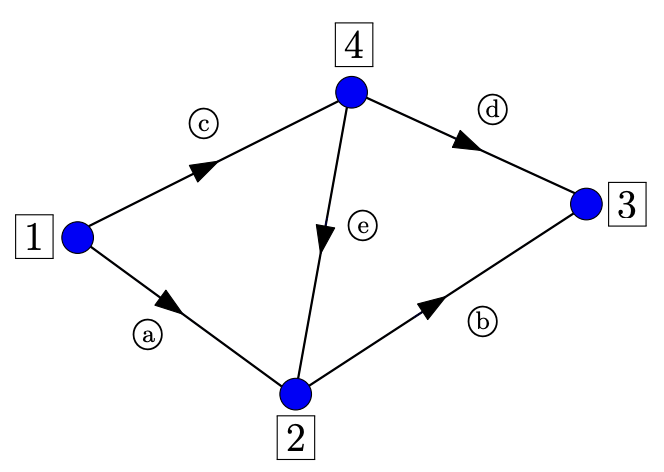
\includegraphics[scale=0.75]{Graph 1}
  \caption{A directed graph with 4 vertices and 5 edges}
\end{figure}
We can construct the so called incidence matrix for this graph as follow:
\begin{definition}[Incidence matrix]
  For a graph \(G=(V,E)\) where \(V=\{v_1,...,v_n\},E=\{e_1,...,e_m\}\), the incidence matrix of an undirected graph is the \(m\times n\) matrix \(B\) whose elements is
  \[b_{ij}=\begin{cases}
    1,& \text{if vertex } v_j \text{ is incident with edge } e_i\\
    0,& \text{otherwise}
  \end{cases}\]
  For directed graph, we have similarly
  \[b_{ij}=\begin{cases}
    -1,& \text{if vertex } v_j \text{ is the head of edge } e_i\\
    1,& \text{if vertex } v_j \text{ is the tail of edge } e_i\\
    0,& \text{otherwise}
  \end{cases}\]
\end{definition}
Note that in some textbook the incidence matrix is defined as the transpose of the one defined here, although it doesn't matter too much.

The incidence matrix of the graph above is thus
\[B=\begin{pmatrix}
  -1 & 1 & 0 & 0 \\
  0 & -1 & 1 & 0 \\
  -1 & 0 & 0 & 1 \\
  0 & 0 & 1 & -1 \\
  0 & 1 & 0 & -1 \\
\end{pmatrix}\]

Observe that 
\[B\begin{pmatrix}1\\1\\1\\1\end{pmatrix}=0:=B\bf{x_0}\]
Hence \(\bf{x_0}\) is a \emph{right null vector}, and is in the \emph{right null space}, or \emph{kernel} of the matrix \(B\). 

Note that the 4 column vectors add to 0, and the first 3 vectors are linearly independent. Hence the dimension of the column space, or the rank of \(A\), is 3. By rank-nullity theorem, the dimension of the kernel is 1.

\vspace{5pt}Observe also that for
\[\bf{w_1}=\begin{pmatrix}1\\0\\-1\\0\\-1\end{pmatrix},\bf{w_2}=\begin{pmatrix}0\\1\\0\\-1\\1\end{pmatrix},\bf{w_3}=\begin{pmatrix}1\\1\\-1\\-1\\0\end{pmatrix}\]
we have \(\bf{w_3}=\bf{w_1}+\bf{w_2}\) and for \(i=1,2,3\),
\[B^\bf{w_i}=(\bf{w_i})^TB=0\]

The vectors \(\bf{w_i}\) are thus in the \emph{left null space} of \(A\). Checking \(\bf{w_1},\bf{w_2}\) are linearly independent and use rank-nullity, we see the dimension of the left null space is 5-3=2.

\vspace{5pt}Now why do we care about this? It turns out that there are nice interpretation of the right and left null space on the graph:
\begin{itemize}
  \item The dimension of the kernel is the number of connected component of a graph. (Thus the vector with component all 1 is always in the kernel)
  \item The dimension of the left null space is the number of closed loops in a graph.
\end{itemize}
We would merely state these informally here without proof, but we can check that this is true with our example above. The graph is connected so \(\dim(\rm{Ker}A)=1\); the number of closed loops is 2, as shown in figure 2.

\begin{figure}[ht]
  \centering
  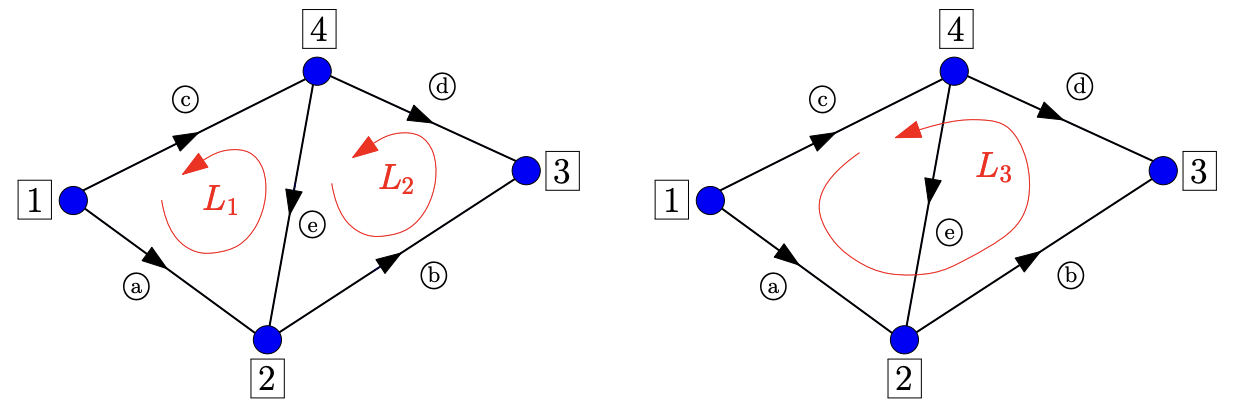
\includegraphics[scale=0.65]{Graph 1 loops}
  \caption{Each loop \(L_i\) corresponds to \(\bf{w_i}\). ``Adding'' \(L_1\) and \(L_2\) is equivalent
  to \(L_3\) since edge \(e\) is effectively not traversed at all.}
\end{figure}

\subsection{Potential and fluxes}
It is often useful to assign values to vertices and edges to represent practical problems better: the value \(x_i\) at vertex \(v_i\) is the \emph{potential} and the value \(w_i\) at edges \(e_i\) is the \emph{flux}. We can get useful information about potential and flux using the incidence matrix.

\begin{proposition}[Potential difference across edge]
  For a graph \(G=(V,E)\) with incidence matrix \(A\) and a column vector \(\bf{x}\) consisting of potential at each vertex, the vector 
  \[\bf{e}=B\bf{x}\]
  gives the difference in potential across each edge (tail minus head).  
\end{proposition}

\begin{proposition}[Net flux out of vertex]
  For a graph \(G=(V,E)\) with incidence matrix \(A\) and a column vector \(\bf{w}\) consisting of flux at each edge, the vector 
  \[\bf{f}=-B^T\bf{w}\]
  gives the total flux diverging out of each vertex.  
\end{proposition}

\subsection{Special matrix}
Let us discuss finally a couple more important matrices before we apply graph theory to some practical scenarios.

\begin{definition}[Degree matrix]
  For a graph \(G=(V,E)\) with \(|V|=n\), the degree matrix \(D\) is the \(n\times n\) matrix
  \[d_{ij}=\begin{cases}
    \deg(v_i),& i=j\\
    0,& i\neq j
  \end{cases}\]
  where \(\deg(v_i)\) is the degree of the vertex, the number of edges incident on it.
\end{definition}

\begin{definition}[Adjacency matrix]
  For a graph \(G=(V,E)\) with \(|V|=n\), the adjacency matrix \(A\) is the \(n\times n\) matrix
  \[a_{ij}=\begin{cases}
    1,& (v_i,v_j)\in E\\
    0,& \text{otherwise} 
  \end{cases}\]
  Here we consider \((v_i,v_j)\) as an unordered pair.
\end{definition}

And finally,
\begin{definition}[Laplacian matrix]
  For a graph \(G=(V,E)\) with \(|V|=n\), the Laplacian matrix \(L\) is the \(n\times n\) matrix
  \[L=D-A\]
\end{definition}

For the graph discussed above, we have
\[D=\begin{pmatrix}
  1 & 0 & 0 & 0 \\
  0 & 3 & 0 & 0 \\
  0 & 0 & 2 & 0 \\
  0 & 0 & 0 & 2 \\
\end{pmatrix}, A=\begin{pmatrix}
  0 & 1 & 0 & 0 \\
  1 & 0 & 1 & 1 \\
  0 & 1 & 0 & 1 \\
  0 & 1 & 1 & 0 \\
\end{pmatrix}, L=\begin{pmatrix}
  1 & -1 & 0 & 0 \\
  -1 & 3 & -1 & -1 \\
  0 & -1 & 2 & -1 \\
  0 & -1 & -1 & 2 \\
\end{pmatrix}\]

\begin{theorem}
  Given a directed graph \(G\) with incidence matrix \(B\) and Laplacian matrix \(L\), we have 
  \[L=B^TB\]
\end{theorem}
For undirected graph, we can assign the direction arbitrarily.

Note also that the Laplacian is symmetric, and the sum of row and column vanishes.

\section{Resistive Circuit Theory}
Let us now study a classical high school electric circuit with our new tools. Through out let the graph have \(n\) vertices and \(m\) edges (unless otherwise stated). We also use the term node and vertex interchangably.

\subsection{Ohm's and Kirchhoff's law}
In resistive circuit theory each edge is assumed to be linear conductor. Then,
\begin{theorem}[Ohm's law]
  Suppose a directed edge (wire) \(e=(v_1,v_2)\) has conductance \(G>0\), flux (current) \(w\), and endpoints have (electric) potential \(x_1,x_2\) respectively, then
  \[w=-G(x_2-x_1)\]
\end{theorem}
Here the conductance is a positive constant depends on the property of the material of the wire. Note also that the \emph{resistance} \(R\) of \(e\) is the inverse of the conductance.

Ohm's law essentially states that the current in the conductor is proportional to the potential difference across it. It is important to note that current flows from high voltage to low voltage: this is the reason for the minus sign.

If we assume unit conductance for all edges, we can write down Ohm's law for a graph with incidence matrix \(B\) as
\[\bf{w}=-\bf{e}=-B\bf{x}\]
where \(\bf{w},\bf{x}\) is the flux and potential vector, respectively.

Recall from earlier that \(\bf{f}=-B^T\bf{w}\), so combine these we have
\[\bf{f}=-B^T(-B\bf{x})=L\bf{x}\]
where \(L\) is the Laplacian and \(\bf{f}\) the vector consisting of net flux out of each vertices.

\begin{theorem}[Kirchhoff's current law]
  If a vertex is not connected to a source or sink, then the net current out of the vertex should be 0. Thus, for a closed system, we have
  \[\bf{f}=0\] 
\end{theorem}

It follows that if the system is closed, we have
\[\bf{f}=-B^T\bf{w}=0 \text{ so } \bf{w}^TB=0\]
This means that the vector of current \(\bf{w}\) must lie in the left null space of \(B\). By rank-nullity theorem, \(\bf{w}\) must be orthogonal to the column space of \(A\), i.e. there is no non-zero potential vector \(\bf{x}\) such that \[\bf{w}=B\bf{x}\]

Hence, in order to have a current in the circuit, we must have Kirchhoff's Current Law (KCL) \emph{not} hold at some vertices. Since \(\bf{f}\) is in the column space of \(A^T\), i.e. the row space of \(A\), and \(\bf{x_0}=(1,...,1)^T\) in the kernel of \(A\), we must have
\[\bf{x}_0^T\bf{f}=\sum_{i=1}^{n}f_i=0\]
where \(f_i,i=1,...,n\) are the entries of \(f\). Hence the net current source must satisfy this. 

\subsection{Two-point source/sink circuit}
Consider the \(n\) dimensional vector \(\bf{f}=(1,-1,0,...,0)^T\). This is the simpliest scenario for a current to exist \((\bf{w}\neq 0)\), where KCL holds at all nodes apart from the first two \emph{boundary nodes}. It is natural to think the first node as a \emph{source} and the second a \emph{sink}. 

\vspace{5pt}\textbf{The Neumann problem}.
The simplest question to ask, given \(\bf{f}\) above, is what is the potential at all nodes, i.e. what's the vector \(\bf{x}\). An example is shown below.

\begin{figure}[ht]
  \centering
  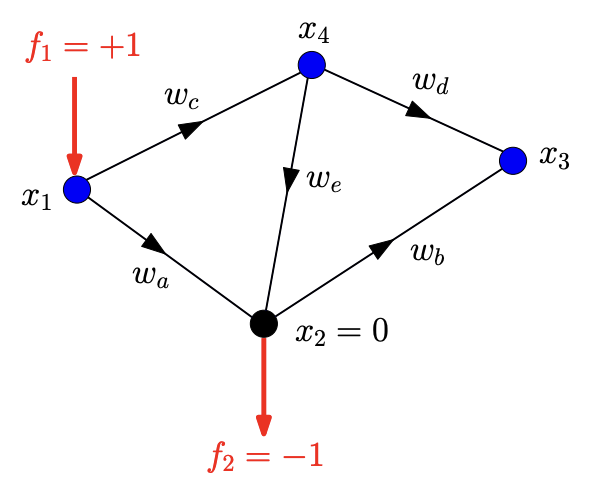
\includegraphics[scale=0.6]{Neumann Problem}
  \caption{The Neumann problem}
\end{figure}

It is tempting to suggest the solution is simply
\begin{equation}\label{eq:1}
  \bf{x}=L^{-1}\bf{f}
\end{equation}
where \(L\) is the Laplacian matrix. Note however, that \(L\) is singular, since \(\bf{x}_0\neq 0\) but
\[L\bf{x}_0=B^TB\bf{x}_0=0\]
as \(\bf{x}_0\) is in the kernel of \(B\). We thus see that if \(\bf{x}\) is a solution to \eqref{eq:1}, then so is \(\bf{x}+c\bf{x}_0\) for any \(c\), corresponding to adding a potential \(c\) to all nodes (which clearly does not change the current since it only depends on the potential difference).

For \(L\) to be not singular, we must remove this freedom. One way of doing this is to \emph{ground} a node, that is, insisting that the potential is 0 at some vertex, say, \(x_2\) in this case. This allow us to remove the 2nd element in the vectors, and the 2nd row and column in the Laplacian, thus allowing us to solve the system via equation \eqref{eq:1}.


\vspace{5pt}\textbf{The Dirichlet problem}.
A similar question is given \(\bf{x}\) instead, what can we say about the vector \(\bf{f}\). Consider this circuit.

\begin{figure}[ht]
  \centering
  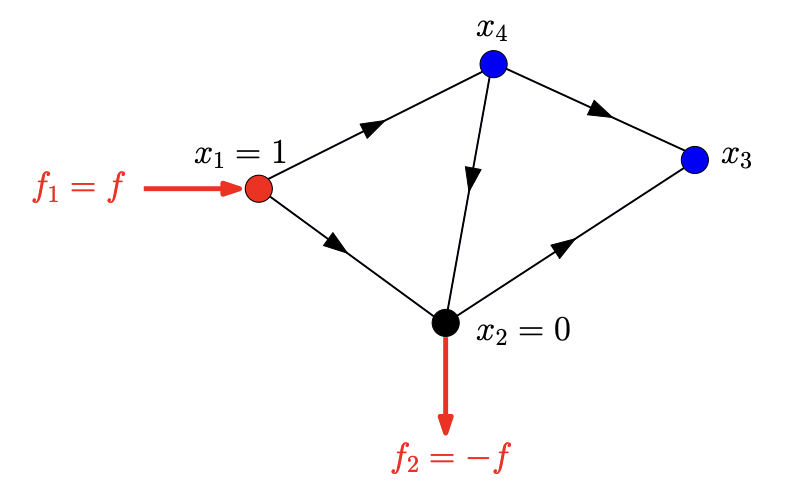
\includegraphics[scale=0.6]{Dirichlet Problem}
  \caption{The Dirichlet problem}
\end{figure} 

We can solve it straight away by a simple scaling if we have already solved the Neumann problem, since the system is linear. 

If we have not, we are left with this equation to solve (KCL holds at \(x_3,x_4\)).
\[L\begin{pmatrix}
  1\\0\\x_3\\x_4
\end{pmatrix}=\begin{pmatrix}
  f\\-f\\0\\0
\end{pmatrix}\]

We may use the method of \emph{Schur complement} for sub-block decomposition.
\begin{definition}[Schur complement]
  Suppose \(p,q\in\N\) and \(A,B,C,D\) are \(p\times p, ..., q\times q\) matrix such that \(M\) is a \((p+q)\times(p+q)\) matrix given by
  \[M=\begin{pmatrix}
    A&B\\C&D
  \end{pmatrix}\]
  If \(D\) is invertible, then the Schur complement of block \(D\) of matrix \(M\) is 
  \[M/D=A-BD^{-1}C\]
  Similary, if \(A\) is invertible, then
  \[M/A=D-CA^{-1}B\]
\end{definition}
Note that Laplacian is symmetric so in these cases we have \(B=C^T\).

Breaking \(\bf{f},\bf{x}\) accordingly will simplify the equation to solve.

\subsection{Conductance matrix}

\begin{definition}[Conductance matrix]
  For a graph \(G=(V,E)\) with \(|E|=m\), the conductance matrix \(C\) is the \(m\times m\) matrix
  \[c_{ij}=\begin{cases}
    c_i,& i=j\\
    0,& i\neq j
  \end{cases}\]
  where \(c_i\) is the conductance of edge \(i\).
\end{definition}

\begin{definition}[Weighted Laplacian]
  For a graph \(G=(V,E)\) with \(|V|=n\), the weighted Laplacian \(L\) is the \(n\times n\) matrix
  \[l_{ij}=\begin{cases}
    -w_{ij},& \text{vertex i,j are connected } \\
    w_i,& i=j\\
    0,& \text{otherwise } 
  \end{cases}\]
  where \(w_{ij}\) is the weight(conductance) of the edge connecting node \(i,j\) and \(w_i\) is the sum of all weights incident on node \(i\).
\end{definition}

\begin{theorem}
  For a graph \(G=(V,E)\) with incidence matrix \(B\), conductance matrix \(C\), the weighted Laplacian \(L\) is given by
  \[L=B^TCB\]
\end{theorem}

\begin{theorem}[Ohm's law with variate conductance]
  For a graph \(G=(V,E)\) with the usual notation, we have
  \[\bf{w}=-C\bf{e}=-CB\bf{x}\]
\end{theorem}
We have still
\[\bf{f}=L\bf{x}\]
except now the Laplacian is weighted.

\subsection{Effective conductance}

\begin{definition}[Effective conductance]
  
\end{definition}

\begin{theorem}[Effective conductance in series]
  In a series circuit (see below), the effective conductance from node 1 to 3 is
  \[C_{eff}=\frac{c_ac_b}{c_a+c_b}\]
\end{theorem}
\begin{figure}[ht]
  \centering
  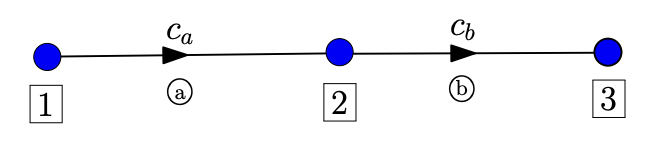
\includegraphics[scale=0.6]{Effective Conductance Series}
  \caption{The simplest series circuit}
\end{figure}

\begin{theorem}[Effective conductance in series]
  In a parallel circuit (see below), the effective conductance from node 1 to 2 is
  \[C_{eff}=c_a+c_b\]
\end{theorem}
\begin{figure}[ht]
  \centering
  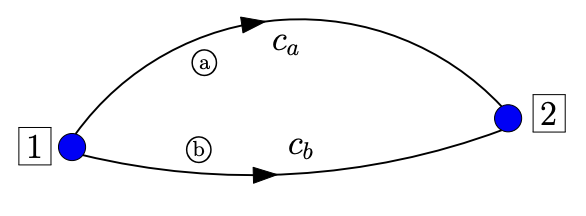
\includegraphics[scale=0.6]{Effective Conductance Parallel}
  \caption{The simplest parallel circuit}
\end{figure}

We have a similar concept of effective resistance, which is used more often in electrical engineering. Since resistance is the inverse of conductance, the formulae above interchange (as learned in high school).

Knowing this, we can often reduce a circuit significantly, such as
\begin{figure}[ht]
  \centering
  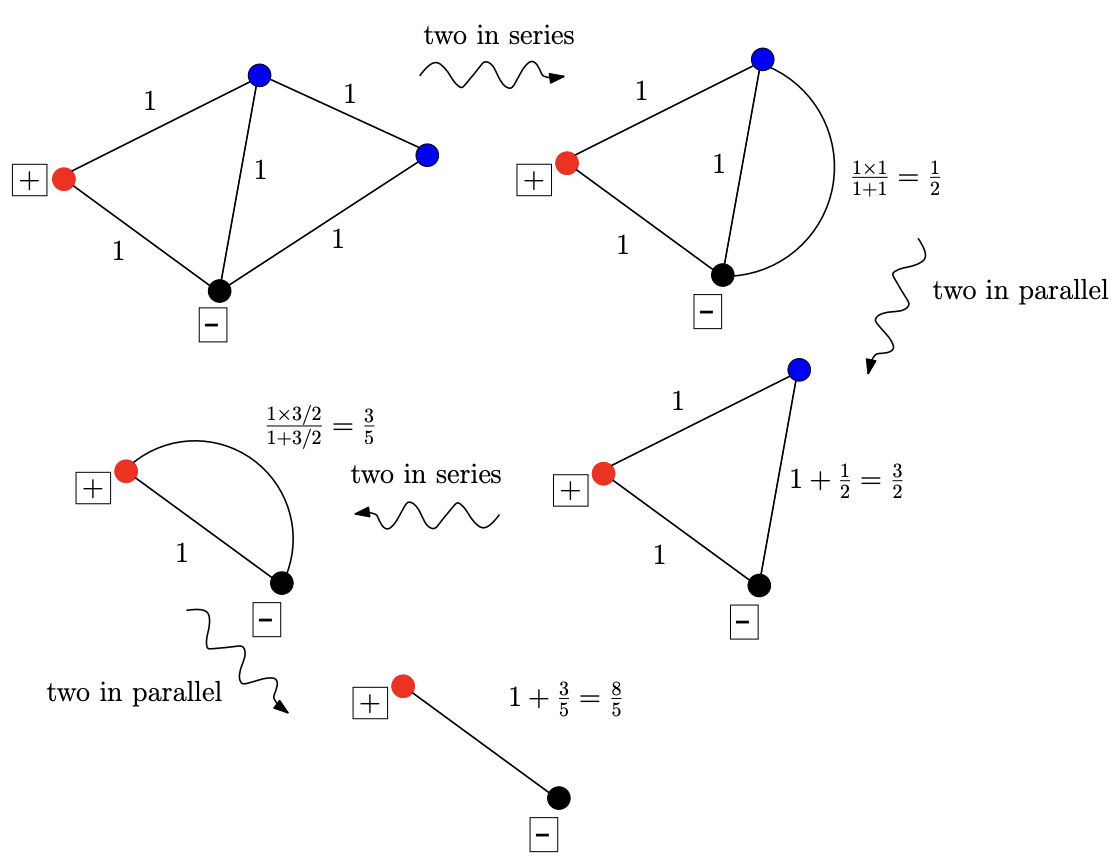
\includegraphics[scale=0.65]{Reducing Circuit}
  \caption{Reducing a circuit via effective conductance}
\end{figure}

\section{Random walk on graph}
\subsection{Some probability}
\subsection{Link with circuit}
\subsection{Energy principles}
\end{document}